\section{تحلیل وابستگی در پایتون و معیارهای جذابیت}

% Slide 30
\begin{frame}[fragile]{تحلیل وابستگی در پایتون}{\lr{Association Analysis in Python}}
\begin{itemize}\setlength{\itemsep}{3pt}
    \item بسته‌ها و کتابخانه‌های متنوعی در پایتون وجود دارند:
    \begin{itemize}\setlength{\itemsep}{2pt}
        \item در تمرین‌ها از بستهٔ \lr{\texttt{Orange3}} استفاده می‌کنیم (و کتابخانهٔ \lr{\texttt{mlxtend}}).
    \end{itemize}
    \vspace{0.15cm}
    \item \textbf{تولید مجموعه‌آیتم‌های مکرر:} {\small (با تعیین حداقل پشتیبان \lr{20\%})}
\end{itemize}

\vspace{-0.1cm}
\begin{center}
\begin{minipage}{0.88\textwidth}
\begin{tcolorbox}[colback=codebg,colframe=codeborder,arc=3pt,left=6pt,right=6pt,top=4pt,bottom=4pt]
\begin{latin}
\fontsize{8.5}{11}\selectfont
\textbf{\color{blue!80!black}{from}} orangecontrib.associate.fpgrowth \textbf{\color{blue!80!black}{import}} frequent\_itemsets\\[3pt]
\textit{\color{gray}{\# Calculate frequent itemsets (min support = 0.20)}}\\
itemsets = dict(frequent\_itemsets(dataset.values, \textbf{\color{red!80!black}{0.20}}))
\end{latin}
\end{tcolorbox}
\end{minipage}
\end{center}

\begin{itemize}\setlength{\itemsep}{3pt}
    \item \textbf{استخراج قواعد وابستگی:} {\small (با تعیین حداقل اطمینان \lr{70\%})}
\end{itemize}

\vspace{-0.1cm}
\begin{center}
\begin{minipage}{0.88\textwidth}
\begin{tcolorbox}[colback=codebg,colframe=codeborder,arc=3pt,left=6pt,right=6pt,top=4pt,bottom=4pt]
\begin{latin}
\fontsize{8.5}{11}\selectfont
\textbf{\color{blue!80!black}{from}} orangecontrib.associate.fpgrowth \textbf{\color{blue!80!black}{import}} association\_rules\\[3pt]
\textit{\color{gray}{\# Calculate association rules from itemsets (min confidence = 0.70)}}\\
rules = association\_rules(itemsets, \textbf{\color{red!80!black}{0.70}})
\end{latin}
\end{tcolorbox}
\end{minipage}
\end{center}
\end{frame}

% Slide 31
\begin{frame}{معیارهای جذابیت قواعد}{\lr{Interestingness Measures}}
\begin{itemize}\setlength{\itemsep}{6pt}
    \item الگوریتم‌های قواعد وابستگی معمولاً \textbf{تعداد بسیار زیادی قاعده} تولید می‌کنند:
    \begin{itemize}\setlength{\itemsep}{3pt}
        \item بسیاری از این قواعد \alert{\textbf{غیرجذاب یا زائد}} \lr{(redundant)} هستند.
        \item یک قاعده زائد است اگر برای مثال $\{A,B,C\} \to \{D\}$ و $\{A,B\} \to \{D\}$ پشتیبان و اطمینان یکسانی داشته باشند.
    \end{itemize}
    \item \textbf{معیارهای جذابیت:} برای هرس کردن، فیلتر یا رتبه‌بندی قواعد تولیدشده به کار می‌روند.
    \item در فرمول‌بندی اولیه، تنها دو معیار \textbf{پشتیبان} و \textbf{اطمینان} استفاده می‌شدند.
    \item بعدها معیارهای تکمیلی متعددی پیشنهاد شدند:
    \begin{itemize}\setlength{\itemsep}{3pt}
        \item در این درس با معیار مهم \textbf{لیفت} \lr{(Lift)} آشنا می‌شویم.
        \item برای مطالعهٔ تفصیلی، مرجع تن و همکاران (فصل ۶.۷) پیشنهاد می‌شود.
    \end{itemize}
\end{itemize}
\end{frame}

% Slide 32
\begin{frame}{نقطهٔ ضعف معیار اطمینان}{\lr{Drawback of Confidence}}
\begin{columns}[T,onlytextwidth]
\begin{column}{0.54\textwidth}
\begin{itemize}\setlength{\itemsep}{2.5pt}\small
    \item \textbf{قاعدهٔ وابستگی:} \lr{Tea $\to$ Coffee}
    \item اطمینان قاعده: $c(\text{Tea} \to \text{Coffee}) = \frac{3}{4} = 0.75$
    \item پشتیبان کل قهوه در داده‌ها: $s(\text{Coffee}) = \frac{18}{20} = 0.90$
    \item با وجود اطمینان بالا (\lr{75\%})، این قاعده \alert{\textbf{گمراه‌کننده}} است؛ زیرا نرخ خریداران قهوه در جامعه (\lr{90\%}) از اطمینان قاعده بیشتر است!
    \item مطلوب است که: $\mathrm{conf}(X \to Y) > \mathrm{supp}(Y)$؛ در غیر این صورت، $X$ شانس رخداد $Y$ را کاهش می‌دهد!
\end{itemize}
\end{column}%
\begin{column}{0.45\textwidth}
\centering
\textbf{\small جدول توافقی}\\[1pt]
{\scriptsize\lr{(Contingency Table)}}\\[3pt]
\begin{latin}
\fontsize{7.5}{9.5}\selectfont
\begin{tabular}{|c|c|c|c|}
\hline
\rowcolor{mannheimblue!15}
 & \textbf{Coffee} & \textbf{$\neg$Coffee} & \textbf{Total} \\ \hline
\textbf{Tea} & 3 & 1 & 4 \\ \hline
\textbf{$\neg$Tea} & 15 & 1 & 16 \\ \hline
\textbf{Total} & 18 & 2 & 20 \\ \hline
\end{tabular}
\end{latin}

\vspace{0.1cm}
\textbf{\small تراکنش‌ها (۲۰ مورد)}\\[3pt]
\begin{latin}
\fontsize{7}{8.5}\selectfont
\begin{tabular}{|c|l|}
\hline
\rowcolor{mannheimblue!15}
\textbf{TID} & \textbf{Items} \\ \hline
1--15 & Coffee \\ \hline
16--18 & Tea, Coffee \\ \hline
19 & Tea \\ \hline
20 & Bread \\ \hline
\end{tabular}
\end{latin}
\end{column}
\end{columns}
\end{frame}

% Slide 33
\begin{frame}{معیار لیفت}{\lr{Lift}}
\begin{itemize}\setlength{\itemsep}{2pt}\small
    \item قاعده‌ای با اطمینان بالا برای $\text{tea} \to \text{coffee}$ کشف کرده‌ایم:
    \begin{itemize}\footnotesize\setlength{\itemsep}{1pt}
        \item \lr{75\%} از افرادی که چای می‌نوشند، قهوه نیز مصرف می‌کنند.
        \item \textbf{فرضیه ذهنی:} افرادی که چای می‌نوشند، تمایل دارند قهوه بنوشند.
        \item \textbf{مفهوم ضمنی:} تمایل آن‌ها \textbf{بیشتر از میانگین کل جامعه} است.
    \end{itemize}
    \item \textbf{آزمون مقایسه:} مقایسهٔ اطمینان قاعده با \textbf{قاعدهٔ پیش‌فرض (پایه):}
    \begin{itemize}\footnotesize\setlength{\itemsep}{1pt}
        \item قاعدهٔ اختصاصی:
        $c_{\text{tea} \to \text{coffee}} = \frac{s(\{\text{tea}\} \cup \{\text{coffee}\})}{s(\{\text{tea}\})}$
        \item قاعدهٔ پیش‌فرض (جامعه):
        $c_{\text{all} \to \text{coffee}} = \frac{s(\text{coffee})}{1} = s(\text{coffee})$
    \end{itemize}
    \item قاعده‌ای را \textbf{پذیرفتنی} می‌دانیم اگر اطمینان آن از قاعدهٔ پیش‌فرض جامعه بیشتر باشد:
    \[
    \frac{c_{\text{tea} \to \text{coffee}}}{c_{\text{all} \to \text{coffee}}} = \frac{c_{\text{tea} \to \text{coffee}}}{s(\text{coffee})} > 1
    \]
\end{itemize}
\end{frame}

% Slide 34
\begin{frame}{تفسیر و ویژگی‌های معیار لیفت}{\lr{Lift}}
\begin{itemize}\setlength{\itemsep}{6pt}
    \item \textbf{تعریف ریاضی لیفت} برای قاعدهٔ $X \to Y$ به صورت زیر است:
    \[
    \mathrm{Lift}(X \to Y) = \frac{c(X \to Y)}{s(Y)} = \frac{s(X \cup Y)}{s(X) \cdot s(Y)}
    \]
    \begin{itemize}\setlength{\itemsep}{2pt}
        \item در واقع: نرمال‌سازی اطمینان قاعده بر حسب پشتیبان مؤخر (نتیجه).
    \end{itemize}
    \vspace{0.2cm}
    \item \textbf{تفسیر آماری لیفت:}
    \begin{itemize}\setlength{\itemsep}{3pt}
        \item \textbf{اگر $\mathrm{Lift} > 1$:} اقلام $X$ و $Y$ دارای \alert{\textbf{همبستگی مثبت}} هستند (خرید $X$ شانس خرید $Y$ را افزایش می‌دهد).
        \item \textbf{اگر $\mathrm{Lift} = 1$:} اقلام $X$ و $Y$ از نظر آماری \textbf{مستقل} هستند ($P(X \cap Y) = P(X)P(Y)$).
        \item \textbf{اگر $\mathrm{Lift} < 1$:} اقلام $X$ و $Y$ دارای \alert{\textbf{همبستگی منفی}} هستند (خرید $X$ مانع خرید $Y$ می‌شود).
    \end{itemize}
\end{itemize}
\end{frame}

% Slide 35
\begin{frame}{مثال محاسبهٔ لیفت}{\lr{Lift (Example)}}
\begin{columns}[T,onlytextwidth]
\begin{column}{0.53\textwidth}
\begin{itemize}\setlength{\itemsep}{3pt}\small
    \item \textbf{قاعدهٔ وابستگی:} \lr{Tea $\to$ Coffee}
    \item اطمینان قاعده: \lr{$c(\text{Tea} \to \text{Coffee}) = \frac{3}{4} = 0.75$}
    \item پشتیبان مؤخر (قهوه): \lr{$s(\text{Coffee}) = \frac{18}{20} = 0.90$}
    \vspace{0.15cm}
    \item \textbf{محاسبهٔ لیفت:}
    \begin{center}
    \begin{latin}
    $\mathrm{Lift}_{\text{Tea} \to \text{Coffee}} = \frac{0.75}{0.90} \approx 0.833 < 1$
    \end{latin}
    \end{center}
    \item \alert{\textbf{نتیجه‌گیری:}} از آنجا که $\mathrm{Lift} < 1$ است، بین مصرف چای و قهوه \textbf{همبستگی منفی} وجود دارد و این قاعده به عنوان قاعده‌ای گمراه‌کننده \textbf{حذف می‌شود}.
\end{itemize}
\end{column}%
\begin{column}{0.45\textwidth}
\centering
\textbf{\small جدول توافقی}\\[1pt]
{\scriptsize\lr{(Contingency Table)}}\\[3pt]
\begin{latin}
\fontsize{7.5}{9.5}\selectfont
\begin{tabular}{|c|c|c|c|}
\hline
\rowcolor{mannheimblue!15}
 & \textbf{Coffee} & \textbf{$\neg$Coffee} & \textbf{Total} \\ \hline
\textbf{Tea} & 3 & 1 & 4 \\ \hline
\textbf{$\neg$Tea} & 15 & 1 & 16 \\ \hline
\textbf{Total} & 18 & 2 & 20 \\ \hline
\end{tabular}
\end{latin}

\vspace{0.1cm}
\textbf{\small تراکنش‌ها (۲۰ مورد)}\\[3pt]
\begin{latin}
\fontsize{7}{8.5}\selectfont
\begin{tabular}{|c|l|}
\hline
\rowcolor{mannheimblue!15}
\textbf{TID} & \textbf{Items} \\ \hline
1--15 & Coffee \\ \hline
16--18 & Tea, Coffee \\ \hline
19 & Tea \\ \hline
20 & Bread \\ \hline
\end{tabular}
\end{latin}
\end{column}
\end{columns}
\end{frame}

% Slide 36
\begin{frame}{سایر معیارهای جذابیت}{\lr{Interestingness Measures}}
\begin{columns}[c,onlytextwidth]
\begin{column}{0.48\textwidth}
\begin{itemize}\setlength{\itemsep}{6pt}
    \item در مقالات و کتب تخصصی داده‌کاوی، \textbf{ده‌ها معیار جذابیت مختلف} پیشنهاد شده است.
    \item برخی از معیارها برای کاربردهای خاصی عالی هستند اما در کاربردهای دیگر عملکرد ضعیفی دارند.
    \item \textbf{مطالعهٔ تفصیلی:} به مراجع تخصصی مراجعه شود (مانند کتاب تن و همکاران، جدول ۶.۱۱).
\end{itemize}
\end{column}%
\begin{column}{0.50\textwidth}
\centering
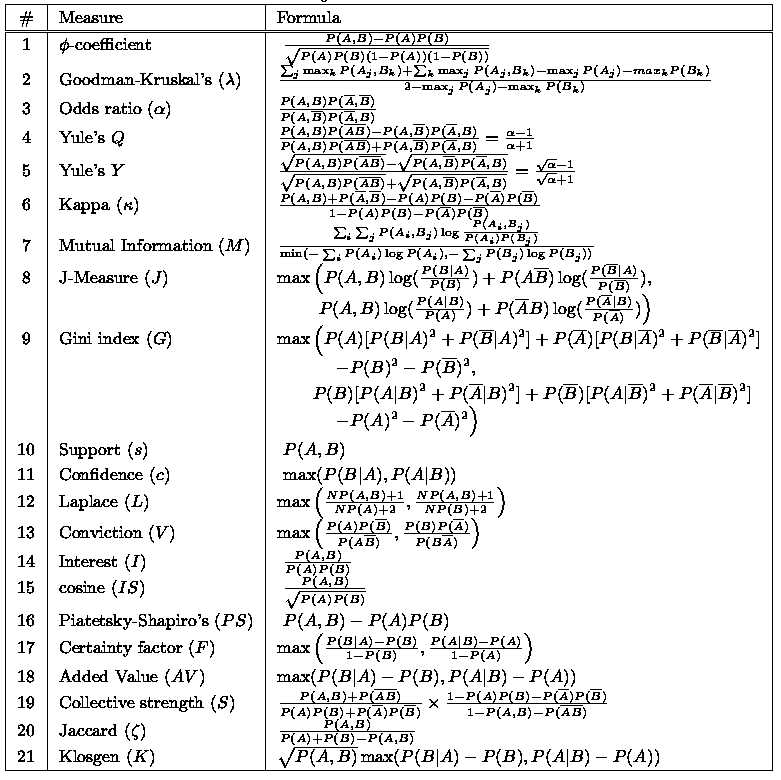
\includegraphics[width=0.98\textwidth,keepaspectratio]{images/extracted_129.png}
\end{column}
\end{columns}
\end{frame}
